\documentclass[border=4pt,12pt]{standalone}
% House style for redrawn exam diagrams (diagram-v4: 0.4pt lines, filled -latex arrows, fine dashes; stipple and hatching drawn as real dots/lines (no PDF/SVG patterns, so they render in every browser and at any scale); transparent background). Every figure \input's this.
\usepackage{amsmath,amssymb}
\usepackage{txfonts}
\usepackage{pdfrender,xcolor}
% \halo{text}: label on shading. The shading stops just around each letter's outline (a thin knock-out that follows the
% glyphs, like the papers' typesetting), never a box. Owner: "I don't want a box around the text".
\newcommand{\halo}[1]{\leavevmode\rlap{\pdfrender{TextRenderingMode=2,LineWidth=2.2pt,LineJoinStyle=1,StrokeColor=white,FillColor=white}#1}#1}
\usepackage{tikz,pgfplots}
\pgfplotsset{compat=1.18}
\usetikzlibrary{arrows.meta,calc,angles,quotes,patterns,patterns.meta,intersections,positioning,decorations.markings,shapes.geometric}
% Stipple and hatching are drawn as actual dots / lines clipped to the region (path picture), NOT as pattern fills:
% SVG <pattern> fills vanish or blur when browsers scale the image, so the owner could not see the shading.
% Each dot is a 0.72pt square (keeps SVGs small; reads as a dot at print size). Dots sit on one global staggered grid, so neighbouring regions line up.
\makeatletter
\newdimen\ex@x \newdimen\ex@y \newdimen\ex@xa \newdimen\ex@ya \newdimen\ex@xb \newdimen\ex@yb \newcount\ex@row
\def\exam@stipplecolor{black!75}\def\exam@dotr{0.42pt}\def\exam@dotgap{2.5}
\def\ex@rowdots{\ifdim\ex@x<\ex@xb \pgfpathrectangle{\pgfqpoint{\dimexpr\ex@x-0.36pt\relax}{\dimexpr\ex@y-0.36pt\relax}}{\pgfqpoint{0.72pt}{0.72pt}}\advance\ex@x by \exam@dotgap pt\relax\expandafter\ex@rowdots\fi}
\def\exam@stipple{%
  \pgftransformreset% dots are sized in real points even inside scaled pictures
  \pgfpointanchor{path picture bounding box}{south west}\ex@xa=\pgf@x \ex@ya=\pgf@y
  \pgfpointanchor{path picture bounding box}{north east}\ex@xb=\pgf@x \ex@yb=\pgf@y
  \pgfsetfillcolor{\exam@stipplecolor}\pgfmathsetmacro\ex@h{\exam@dotgap/2}%
  \pgfmathtruncatemacro\ex@r{floor(\ex@ya/\ex@h)-1}\ex@row=\ex@r\relax
  \ex@y=\ex@r\dimexpr\ex@h pt\relax
  \loop\ifdim\ex@y<\ex@yb
    \pgfmathtruncatemacro\ex@c{floor(\ex@xa/\exam@dotgap)-1}\ex@x=\ex@c\dimexpr\exam@dotgap pt\relax
    \ifodd\ex@row \advance\ex@x by \ex@h pt\fi
    \ex@rowdots
    \advance\ex@y by \ex@h pt \advance\ex@row by 1
    \ifnum\numexpr\ex@row-(\ex@row/4)*4\relax=0 \pgfusepath{fill}\fi% flush every 4 rows: bounded TeX memory, few clip copies in the SVG
  \repeat\pgfusepath{fill}}
\newdimen\ex@d
\def\exam@hatch#1{% #1 = 1 for /, -1 for \ ; lines 45 degrees, 3pt apart
  \pgftransformreset
  \pgfpointanchor{path picture bounding box}{south west}\ex@xa=\pgf@x \ex@ya=\pgf@y
  \pgfpointanchor{path picture bounding box}{north east}\ex@xb=\pgf@x \ex@yb=\pgf@y
  \ex@d=\dimexpr\ex@yb-\ex@ya\relax \ex@x=\dimexpr\ex@xa-\ex@d\relax
  \loop\ifdim\ex@x<\ex@xb
    \ifnum#1>0 \pgfpathmoveto{\pgfqpoint{\ex@x}{\ex@ya}}\pgfpathlineto{\pgfqpoint{\dimexpr\ex@x+\ex@d\relax}{\ex@yb}}%
    \else \pgfpathmoveto{\pgfqpoint{\ex@x}{\ex@yb}}\pgfpathlineto{\pgfqpoint{\dimexpr\ex@x+\ex@d\relax}{\ex@ya}}\fi
    \advance\ex@x by 4.24pt
  \repeat
  \pgfsetlinewidth{0.4pt}\pgfsetstrokecolor{black}\pgfusepath{stroke}}
\def\examstipple{\exam@stipple}\def\examhatch{\exam@hatch}\def\examsetstipplecolor#1{\def\exam@stipplecolor{#1}}\def\examsetdotgap#1{\def\exam@dotgap{#1}}
\makeatother
% (legacy pattern kept for old files)
% staggered stipple like the NESA papers' dotted shading
\pgfdeclarepatternformonly{exam stipple}{\pgfpointorigin}{\pgfqpoint{2.2pt}{2.2pt}}{\pgfqpoint{2.2pt}{2.2pt}}{%
  \pgfpathcircle{\pgfqpoint{0.55pt}{0.55pt}}{0.42pt}\pgfpathcircle{\pgfqpoint{1.65pt}{1.65pt}}{0.42pt}\pgfusepath{fill}}
\tikzset{
  every picture/.style={line width=0.6pt, >={Latex[length=2mm,width=1.3mm]}},
  curve/.style={line width=0.6pt},
  open arrow/.style={-{Latex[length=2mm,width=1.3mm]}},  % owner: filled -latex heads everywhere, no open chevrons
  aux/.style={dash pattern=on 2pt off 1.5pt, line width=0.6pt},
  shade/.code={\def\exA{#1}\def\exB{none}\ifx\exA\exB\else\pgfkeysalso{fill=black!18}\fi},
  shade/.default=on,
  shade dots/.style={fill=none, path picture={\examstipple}},
  stipple color/.code={\examsetstipplecolor{#1}},
  stipple gap/.code={\examsetdotgap{#1}},
  shade dense dots/.style={fill=none, stipple gap=1.6, path picture={\examstipple}},
  shade hatch/.style={fill=none, path picture={\examhatch{1}}},
  shade hatch reverse/.style={fill=none, path picture={\examhatch{-1}}},
  shade solid/.style={fill=black},
  pt/.style={circle, fill, inner sep=1.1pt},
  open pt/.style={circle, draw, fill=white, inner sep=1.1pt},
}
\pgfplotsset{
  exam axes/.style={axis lines=middle, axis line style={->}, xlabel={$x$}, ylabel={$y$},
    xlabel style={anchor=west}, ylabel style={anchor=south}, tick label style={font=\small},
    every axis plot/.append style={line width=0.6pt, black}, samples=200, clip=false,
    enlargelimits=false, axis on top},
}

\begin{document}
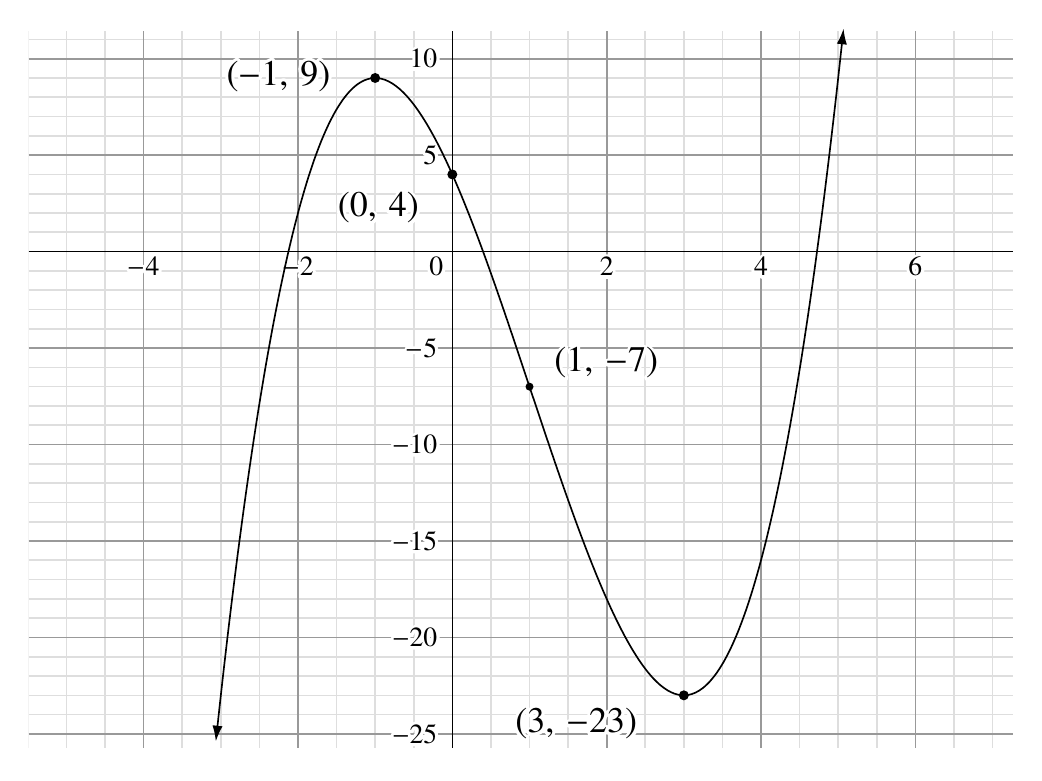
\begin{tikzpicture}[x=0.0127cm,y=-0.0127cm,every node/.style={font=\fontsize{10}{12}\selectfont}]
\begin{scope}\clip (5,5) rectangle (990,722);
\draw[black!13] (4.4,5) -- (4.4,722);
\draw[black!13] (43.0,5) -- (43.0,722);
\draw[black!13] (81.6,5) -- (81.6,722);
\draw[black!13] (158.8,5) -- (158.8,722);
\draw[black!13] (197.4,5) -- (197.4,722);
\draw[black!13] (236.0,5) -- (236.0,722);
\draw[black!13] (313.2,5) -- (313.2,722);
\draw[black!13] (351.8,5) -- (351.8,722);
\draw[black!13] (390.4,5) -- (390.4,722);
\draw[black!13] (467.6,5) -- (467.6,722);
\draw[black!13] (506.2,5) -- (506.2,722);
\draw[black!13] (544.8,5) -- (544.8,722);
\draw[black!13] (622.0,5) -- (622.0,722);
\draw[black!13] (660.6,5) -- (660.6,722);
\draw[black!13] (699.2,5) -- (699.2,722);
\draw[black!13] (776.4,5) -- (776.4,722);
\draw[black!13] (815.0,5) -- (815.0,722);
\draw[black!13] (853.6,5) -- (853.6,722);
\draw[black!13] (930.8,5) -- (930.8,722);
\draw[black!13] (969.4,5) -- (969.4,722);
\draw[black!13] (1008.0,5) -- (1008.0,722);
\draw[black!13] (5,785.2) -- (990,785.2);
\draw[black!13] (5,765.9) -- (990,765.9);
\draw[black!13] (5,746.6) -- (990,746.6);
\draw[black!13] (5,727.3) -- (990,727.3);
\draw[black!13] (5,688.7) -- (990,688.7);
\draw[black!13] (5,669.4) -- (990,669.4);
\draw[black!13] (5,650.1) -- (990,650.1);
\draw[black!13] (5,630.8) -- (990,630.8);
\draw[black!13] (5,592.2) -- (990,592.2);
\draw[black!13] (5,572.9) -- (990,572.9);
\draw[black!13] (5,553.6) -- (990,553.6);
\draw[black!13] (5,534.3) -- (990,534.3);
\draw[black!13] (5,495.7) -- (990,495.7);
\draw[black!13] (5,476.4) -- (990,476.4);
\draw[black!13] (5,457.1) -- (990,457.1);
\draw[black!13] (5,437.8) -- (990,437.8);
\draw[black!13] (5,399.2) -- (990,399.2);
\draw[black!13] (5,379.9) -- (990,379.9);
\draw[black!13] (5,360.6) -- (990,360.6);
\draw[black!13] (5,341.3) -- (990,341.3);
\draw[black!13] (5,302.7) -- (990,302.7);
\draw[black!13] (5,283.4) -- (990,283.4);
\draw[black!13] (5,264.1) -- (990,264.1);
\draw[black!13] (5,244.8) -- (990,244.8);
\draw[black!13] (5,206.2) -- (990,206.2);
\draw[black!13] (5,186.9) -- (990,186.9);
\draw[black!13] (5,167.6) -- (990,167.6);
\draw[black!13] (5,148.3) -- (990,148.3);
\draw[black!13] (5,109.7) -- (990,109.7);
\draw[black!13] (5,90.4) -- (990,90.4);
\draw[black!13] (5,71.1) -- (990,71.1);
\draw[black!13] (5,51.8) -- (990,51.8);
\draw[black!13] (5,13.2) -- (990,13.2);
\draw[black!13] (5,-6.1) -- (990,-6.1);
\draw[black!13] (5,-25.4) -- (990,-25.4);
\draw[black!13] (5,-44.7) -- (990,-44.7);
\draw[black!40] (-34.2,5) -- (-34.2,722);
\draw[black!40] (120.2,5) -- (120.2,722);
\draw[black!40] (274.6,5) -- (274.6,722);
\draw[black!40] (429.0,5) -- (429.0,722);
\draw[black!40] (583.4,5) -- (583.4,722);
\draw[black!40] (737.8,5) -- (737.8,722);
\draw[black!40] (892.2,5) -- (892.2,722);
\draw[black!40] (1046.6,5) -- (1046.6,722);
\draw[black!40] (5,804.5) -- (990,804.5);
\draw[black!40] (5,708.0) -- (990,708.0);
\draw[black!40] (5,611.5) -- (990,611.5);
\draw[black!40] (5,515.0) -- (990,515.0);
\draw[black!40] (5,418.5) -- (990,418.5);
\draw[black!40] (5,322.0) -- (990,322.0);
\draw[black!40] (5,225.5) -- (990,225.5);
\draw[black!40] (5,129.0) -- (990,129.0);
\draw[black!40] (5,32.5) -- (990,32.5);
\draw[black!40] (5,-64.0) -- (990,-64.0);
\end{scope}
\draw (5,225.5) -- (990,225.5); \draw (429,5) -- (429,722);
\node at (120.2,240.5) {\halo{$-4$}};
\node at (274.6,240.5) {\halo{$-2$}};
\node at (583.4,240.5) {\halo{$2$}};
\node at (737.8,240.5) {\halo{$4$}};
\node at (892.2,240.5) {\halo{$6$}};
\node at (413.0,240.5) {\halo{$0$}};
\node[anchor=east] at (424.0,32.5) {\halo{$10$}};
\node[anchor=east] at (424.0,129.0) {\halo{$5$}};
\node[anchor=east] at (424.0,322.0) {\halo{$-5$}};
\node[anchor=east] at (424.0,418.5) {\halo{$-10$}};
\node[anchor=east] at (424.0,515.0) {\halo{$-15$}};
\node[anchor=east] at (424.0,611.5) {\halo{$-20$}};
\node[anchor=east] at (424.0,708.0) {\halo{$-25$}};
\draw[<->] plot[domain=-3.065:5.07, smooth, samples=90] ({429+77.2*\x},{225.5-19.3*(\x*\x*\x-3*\x*\x-9*\x+4)});
\fill (351.8,51.8) circle (5);
\fill (429.0,148.3) circle (5);
\fill (506.2,360.6) circle (4);
\fill (660.6,669.4) circle (5);
\node[font=\fontsize{13}{15}\selectfont] at (255,50) {\halo{$(-1,\,9)$}};
\node[font=\fontsize{13}{15}\selectfont] at (355,182) {\halo{$(0,\,4)$}};
\node[font=\fontsize{13}{15}\selectfont] at (583,337) {\halo{$(1,\,-7)$}};
\node[font=\fontsize{13}{15}\selectfont] at (553,698) {\halo{$(3,\,-23)$}};
\end{tikzpicture}
\end{document}
